\section{Application 3} \label{sec:case_study3}

This section presents and compares the results of the three conducted experiments. In Section~\ref{subsec:dualdec}, the proposed model is compared with other models with dual decomposition but without the use of \ac{STACK}. In Section~\ref{subsec:singledec}, the performance of the proposed model is compared with the performance of models with a single-stage decomposition using \ac{VMD} and \ac{SSA}. Section~\ref{subsec:nondec} compares the proposed model with non-decomposed models, the last experiment. Through these experiments, the forecasting accuracy of the proposed model can be effectively assessed and compared. From Tables \ref{tab:vmd-ssa} to \ref{tab:single} on Appendix~\ref{app:hyper3}, the best results are highlighted in bold.

\subsection{Comparison with dual decomposed models \label{subsec:dualdec}}

The model proposed in this work for wind speed forecast is based on dual decomposition by \ac{VMD} and \ac{SSA} in conjunction with \ac{STACK}. In this first experiment, the proposed model (\ac{VMD}--\ac{SSA}--\ac{STACK}) is compared to the other four models that use dual decomposition, namely \ac{VMD}--\ac{SSA}--\ac{KNN}, \ac{VMD}--\ac{SSA}--\ac{PLS}, \ac{VMD}--\ac{SSA}--\ac{RIDGE}, and \ac{VMD}--\ac{SSA}--\ac{SVR}. The \ac{STACK} method is not used in these models, just the dual decomposition. The results of these models were the ones used as inputs for the proposed \ac{VMD}--\ac{SSA}--\ac{STACK} model. Comparisons are made for all models, in every time horizon, and for all datasets. Furthermore, the model proposed by \citeonline{moreno2020Multistep} (\ac{VMD}--\ac{SSA}--LSTM) was also compared.

Within this first comparison, presented in Table \ref{tab:vmd-ssa}, the \ac{VMD}--\ac{SSA}--\ac{STACK} model outperformed all other compared models. The least accurate model for March 2020 was the \ac{VMD}--\ac{SSA}--\ac{SVR} for all time horizons in all performance criteria, except the \ac{RMSE} when forecasting 10 minutes, while \ac{VMD}--\ac{SSA}--\ac{KNN} was the least accurate model. For April and May 2020, in all forecasting horizons, regarding all performance criteria, the \ac{VMD}--\ac{SSA}--\ac{KNN} was the least accurate model, with an \ac{IP} that ranges from 14.99 to 32.73\%, when compared to \ac{VMD}--\ac{SSA}--\ac{STACK}. On the other hand, \ac{VMD}--\ac{SSA}--\ac{PLS} was the second most accurate model regarding March 2020 forecasting 10 minutes, April and May 2020 forecasting 10 and 30 minutes ahead. For the remaining scenarios, i.e., March 2020, for 30 and 60 minutes, and April and May 2020, for 60 minutes, the \ac{VMD}--\ac{SSA}--\ac{RIDGE} was the second most accurate model.

\textbf{Remark:} The proposed forecasting model outperformed the evaluated \ac{VMD}--\ac{SSA} models, even though the dual decomposition approach presented low errors (\ac{MAPE} $< 8\%$) and was effectively performed by \citeonline{moreno2020Multistep} and \citeonline{moreno2021Hybrid}. This result is due to the divide-and-conquer approach that the \ac{STACK} method provides. The main gain of the \ac{STACK} approach is its ability to take advantage of all different learning strategies of every forecasting base model and use it in conjunction to forecast as accurately as possible. Thus, the higher the diversity of the base models, the stronger the \ac{STACK} becomes, i.e., the variety of the ensemble is more important than the number of models composing the ensemble, as explained by \citeonline{ribeiro2020Ensemble}. Hence, even though the \ac{VMD}--\ac{SSA}--\ac{KNN} model is not very accurate, its learning characteristics enhance the learning process of the ensemble as a whole.

\subsection{Comparison with single decomposed models \label{subsec:singledec}}
Compared to the proposed forecasting model, the second experiment evaluates the single decomposed models, performed by \ac{VMD} and \ac{SSA} approaches. The \ac{VMD}-based models are named \ac{VMD}--\ac{STACK}, \ac{VMD}--\ac{KNN}, \ac{VMD}--\ac{PLS}, \ac{VMD}--\ac{RIDGE}, and \ac{VMD}--\ac{SVR}, and the \ac{SSA}-based models are named \ac{SSA}--\ac{STACK}, \ac{SSA}--\ac{KNN}, \ac{SSA}--\ac{PLS}, \ac{SSA}--\ac{RIDGE}, and \ac{SSA}--\ac{SVR}. The performance metrics of these models are presented in Tables \ref{tab:vmd} and \ref{tab:ssa}, respectively.

Regarding the \ac{VMD} models, presented in Table \ref{tab:vmd}, the proposed approach outperformed the evaluated models in every dataset for all horizons. Analyzing the March 2020 dataset, the \ac{VMD}--\ac{SVR} was the most petite accurate model in each forecasting horizon, while the \ac{VMD}--\ac{STACK} was the second most precise model for forecasting 10 minutes, and the \ac{VMD}--\ac{RIDGE} 30 and 60 minutes ahead. Regarding April and May 2020 datasets, for all forecasting horizons and all performance criteria, the \ac{VMD}--\ac{KNN} and \ac{VMD}--\ac{RIDGE} models were the least and most accurate models, respectively. 

Further, regarding the \ac{SSA} models, presented in Table \ref{tab:ssa}, the \ac{VMD}--\ac{SSA}--\ac{STACK} was the most accurate model for all datasets in all forecasting horizons with an \ac{IP} that ranges between 3.29--81.54\%. For this experiment, the second-most precise model, respectively, was (i) the \ac{SSA}--\ac{STACK} for March 2020 for 10 minutes ahead, and April and May 2020 for 60 minutes ahead; (ii) the \ac{SSA}--\ac{RIDGE} for March 2020 for 30 and 60 minutes, April 2020 for 10 and 30 minutes, and May 2020 for 10 minutes ahead; and (iii) \ac{SSA}--\ac{PLS} when forecasting 30 minutes in May 2020 dataset. Besides, the least accurate model was the \ac{SSA}--\ac{KNN} model for all datasets and forecasting horizons, except for May 2020 when forecasting 60 minutes, in which \ac{SSA}--\ac{SVR} was the least accurate model.

\textbf{Remark:} Indeed, \ac{VMD} and \ac{SSA} are effective preprocessing techniques to forecast wind speed time series multi-step-ahead, as presented by \citeonline{zhang2020Adaptive} and \citeonline{hu2021Wind} (who proposed \ac{VMD}-based models to forecast wind speed), and \citeonline{liu2019Smart} who proposed \ac{SSA}-based model. Despite the consistently accurate performance of \ac{VMD} and \ac{SSA}-based models \cite{moreno2018Wind, zhang2021Hybrid} and the characteristics of the \ac{STACK} to potentialize the forecasting, they were not able to overcome the hybridization of the three approaches presented in the \ac{VMD}--\ac{SSA}--\ac{STACK} model. This result is because the \ac{VMD} technique extracted the trend component from the original time series, and the \ac{SSA} approach denoised the remaining signal. That enables the training models to deal with the high and low frequencies of the time series. Also, same as the previous experiment, the \ac{STACK} scheme enhanced the whole forecasting process.

\subsection{Comparison with the non-decomposed models \label{subsec:nondec}}
The final experiment compared the proposed approach to models that do not use decomposition. These models were \ac{STACK}, \ac{KNN}, \ac{PLS}, \ac{RIDGE}, \ac{SVR}, \ac{ANN}, \ac{ESN}, and \ac{LSTM}. The performance metrics of those five models are presented in Table~\ref{tab:single}.

Like the previous comparisons, the proposed forecasting model outperformed the non-decomposed machine learning and \ac{STACK} models for all scenarios in all performance metrics. The \ac{IP} ranged between 5.57--99.08\%, with the \ac{KNN} model being the least accurate model in all scenarios, except for April 2020 for 60 minutes, while the \ac{STACK} model presented the least accurate performance.

\textbf{Remark:} Although the non-decomposed models usually could not deal with nonlinearity and non-stationary behavior of the wind speed data, these models presented satisfactory results since the \ac{MAPE} criteria of them were not higher than 13\%. Even with promising results related to the non-decomposed models, they could not overcome the \ac{VMD}--\ac{SSA}--\ac{STACK} model. On the other hand, it is essential to emphasize that these models compose the proposed forecasting framework. When these methods are combined, it is possible to build an accurate and efficient forecasting model from the different characteristics and strategies of the approaches.

\subsection{Hypothesis tests and graphical analysis \label{subsec:hypothesis}}

The \ac{DM} test was used to compare the top-performing model regarding the performance metrics solely with other models. The hypothesis test was performed by comparing the proposed model with all other models in each dataset in all forecasting horizons. Table \ref{tab:dm} on Appendix~\ref{app:hyper3} shows the \ac{DM} statistic for all comparisons, highlighting the statistical significance in which the null hypothesis is rejected. The \ac{DM} test results show that the proposed model performed better than all models in all given scenarios once all the statistics presented negative values, and most of them showed $p$-values lower than 0.01.

Regarding the \ac{DM} statistics and $p$-values of the analysis, it is possible to notice that (i) for March 2020 forecasting 10 minutes ahead, the \ac{VMD}--\ac{SSA}--\ac{STACK} is statistically equal to the \ac{VMD}--\ac{SSA}--\ac{PLS} and \ac{VMD}--\ac{SSA}--\ac{RIDGE} models; (ii) for March 2020 forecasting 60 minutes ahead, the \ac{VMD}--\ac{SSA}--\ac{STACK} is statistically equal to \ac{VMD}--\ac{SSA}--\ac{RIDGE}; and (iii) for all other datasets and forecasting horizons, the \ac{VMD}--\ac{SSA}--\ac{STACK} is statistically different from the other models. It is important to emphasize that even for the models where the difference was not statistically significant with a significance of 5\%, the proposed model performed better in all performance metrics.

Using Equation \eqref{eq:ip}, it was possible to calculate the \ac{IP} of each forecasting model compared to the most accurate model, according to each performance criterion. All models have been compared to \ac{VMD}--\ac{SSA}--\ac{STACK}, and their respective \ac{IP} (in percentage) are presented in Tables \ref{tab:ip1} and \ref{tab:ip2} on Appendix~\ref{app:hyper3}. The lower the \ac{IP}, the closer the model's performance is to the proposed model. Note that once the \ac{VMD}--\ac{SSA}--\ac{STACK} model is the most accurate model for all scenarios, its \ac{IP} is always 0\%. 

After calculating each forecasting model's average \ac{IP}, it was possible to rank the models according to their performance compared to the most accurate model of each dataset in each forecasting horizon. Figure~\ref{fig:ip} presents the models ranked according to the average \ac{IP} of every dataset for all forecasting horizons from the most to the least accurate model.

% Figure - Average IP
\begin{figure}[htb!]
    \centering
    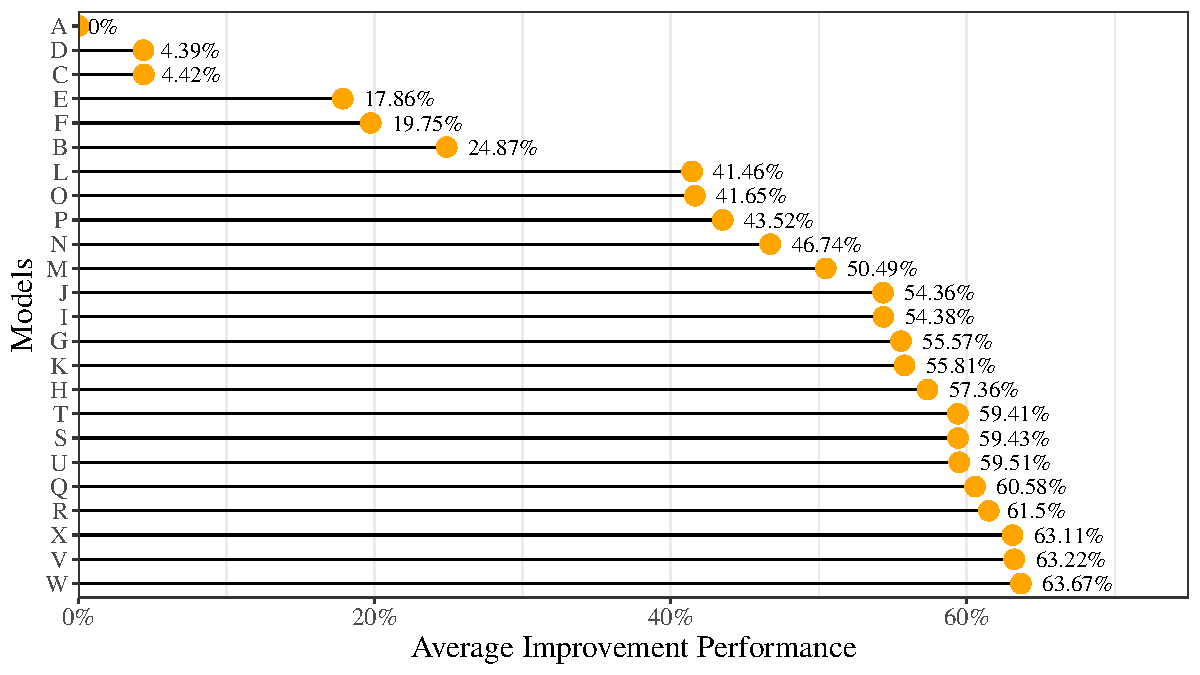
\includegraphics[width=.9\linewidth]{Media/cs3_avr_ip.pdf}
    \caption{Average improvement performance of each evaluated forecasting model}
    \label{fig:ip}
    \source{\citeonline{dasilva2022Multistep}}
\end{figure}

As analyzed in Tables~\ref{tab:vmd-ssa} to \ref{tab:dm}, and Figure~\ref{fig:ip}, the \ac{VMD}--\ac{SSA}--\ac{STACK} and \ac{KNN} are the most and least accurate models, respectively. Besides, we can notice that \ac{VMD}--\ac{SSA}-based models performed better than other compared models. Ranking the evaluated approaches, then the dual decomposition approach presented better performance. After that, single decomposition approaches (\ac{SSA} and \ac{VMD}, in this order), and last, the non-decomposed models. Indeed, it is evident that the combination of the two decomposition approaches performed better than the other approaches.

These results are due to the \ac{VMD} method, which deals with the non-linear and non-stationary behaviors of wind speed data, completely neutralizing the residual noise, producing an improved method \cite{dasilva2020Forecasting}. Also, the results are enhanced due to the \ac{SSA} approach, a powerful non-parametric method for processing non-stationary signals and valuable for filtering the low-frequency noise \cite{moreno2020Multistep}. In addition, due to the divide-and-conquer approach of the \ac{STACK} method, the proposed model takes advantage of the different learning strategies of each model and uses its best to forecast more accurately \cite{dasilva2020Multistep}. The combination of the strengths of these approaches made it possible to outperform the \ac{SSA}, \ac{VMD}, and especially the single models.

In Figure \ref{fig:radarplot}, the standard deviation of the errors of each forecasting model evaluated in all forecasting horizons analyzed is shown in a radar plot. The closer the line is to the center of the radar, the smaller the standard deviation of the respective model's error, showing how accurate that model is. In this figure, the models are labeled the same way as in Table \ref{tab:dm} and Figure \ref{fig:ip}. It is possible to observe that the proposed \ac{VMD}--\ac{SSA}--\ac{STACK} model (A) showed the lowest errors in every case, evidence that the model learned better than all other compared models.

% Figure - Radar
\begin{figure}[htb!]
    \centering
    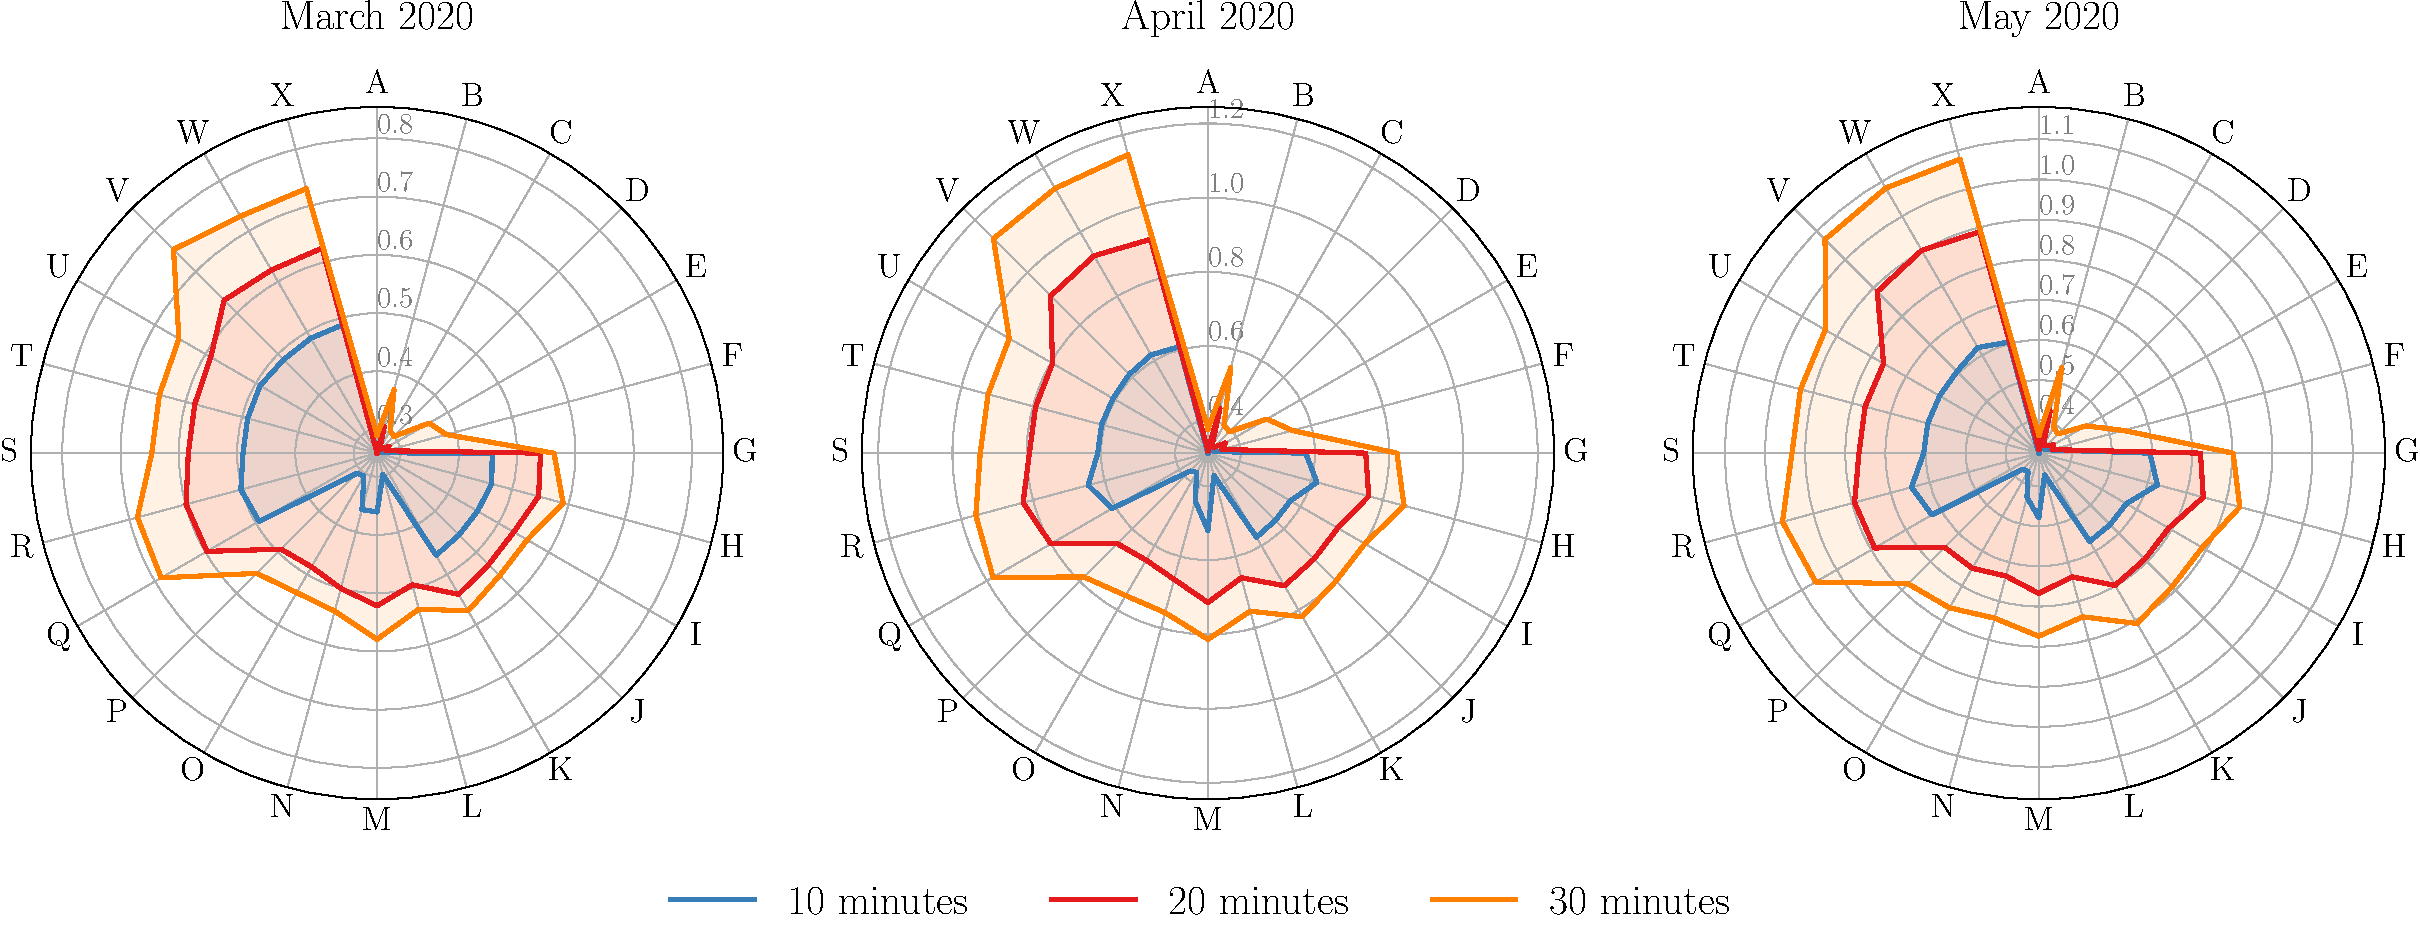
\includegraphics[width=\linewidth]{Media/cs3_radarplot.pdf}
    \caption{Errors' standard deviation for each evaluated forecasting model}
    \label{fig:radarplot}
    \source{\citeonline{dasilva2022Multistep}}
\end{figure}

Moreover, according to the presented performance metrics, hypothesis tests, and the graphical statistical analysis, the \ac{VMD}--\ac{SSA}--\ac{STACK} was the most accurate model for all datasets (March, April, and May 2020) in all evaluated forecasting horizons (10, 30, and 60 minutes ahead). Due to the amount of data and to facilitate the visualization of the relationship between the observed and predicted values, Figure \ref{fig:po} presented the last 24 hours of observation (last 144 observations) in blue versus the predictions in red for 10, 30, and 60-minutes ahead, for March, April, and May 2020.

% Figure - PO
\begin{figure}[htb!]
    \centering
    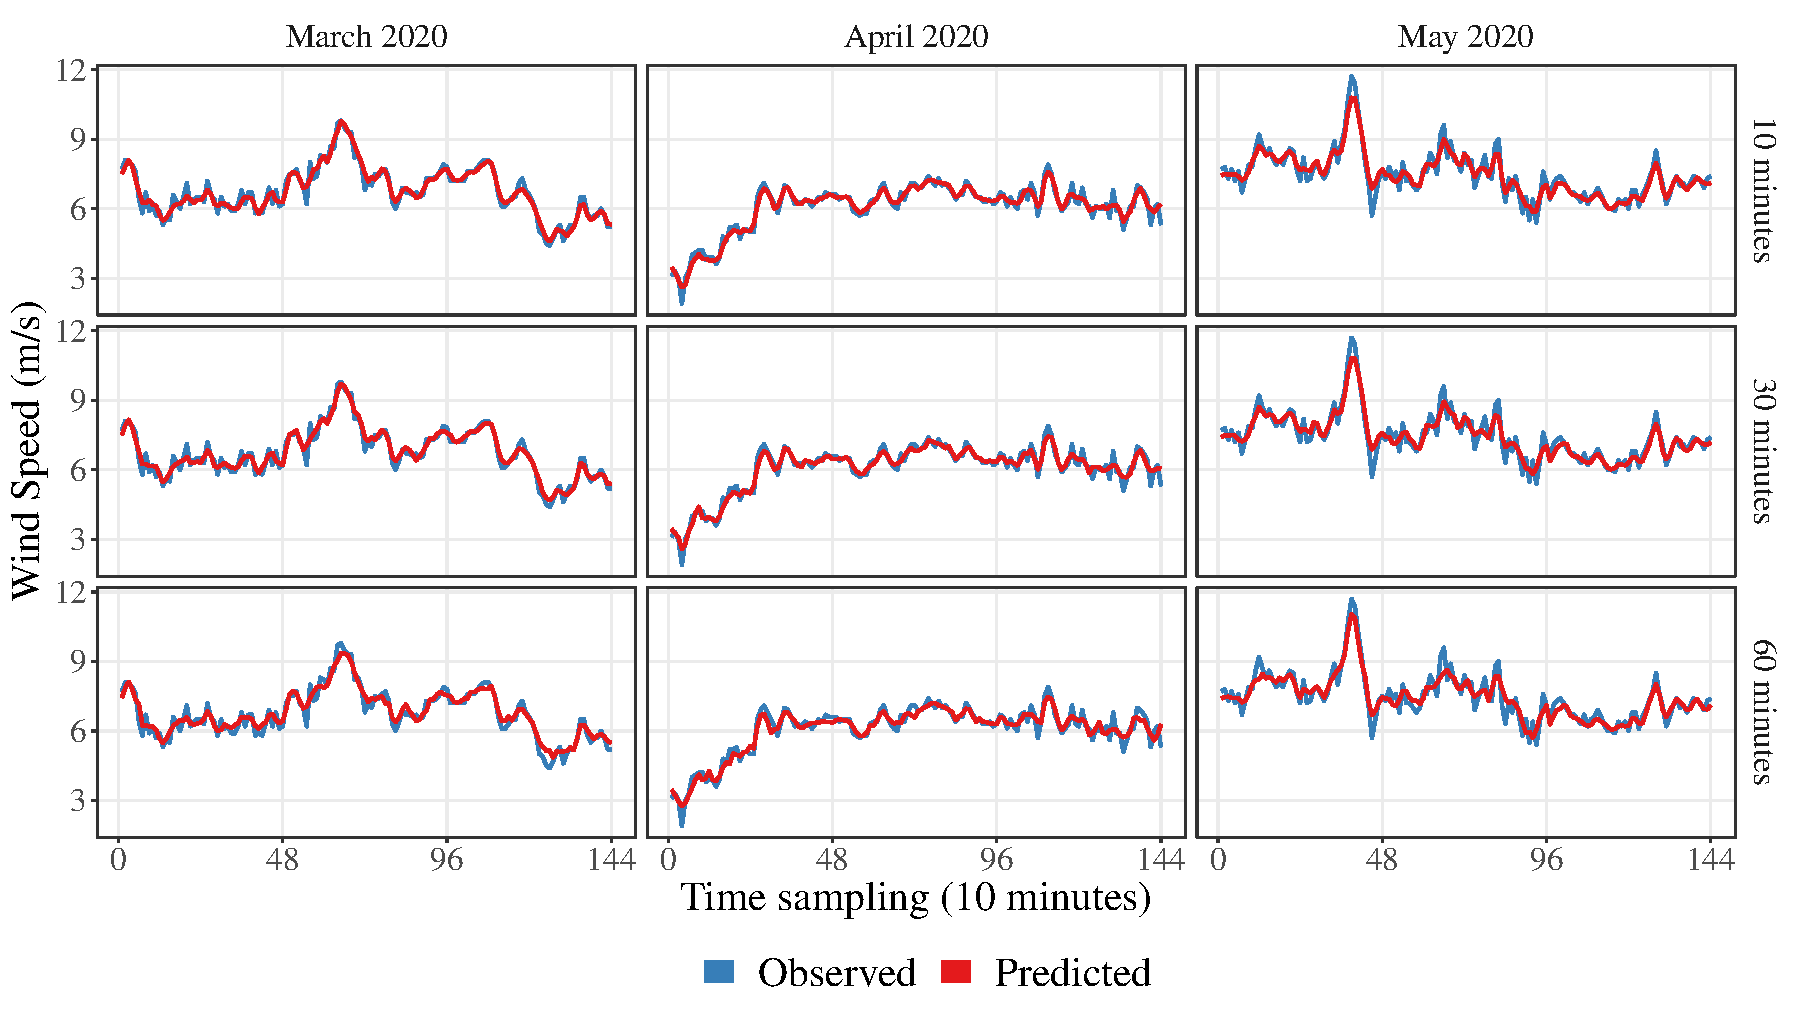
\includegraphics[width=\linewidth]{Media/cs3_PO.pdf}
    \caption{Observed versus predicted time series for the last 24 hours of all datasets in all forecasting horizons}
    \label{fig:po}
    \source{\citeonline{dasilva2022Multistep}}
\end{figure}

Regarding the predicted versus observed values of the wind speed ($m/s$), the proposed forecasting framework learned the data behavior, which in turn made it able to predict accurate values compatible with the ones from the observed time series. Even in the extremes of the data variability in longer forecasting horizons (i.e., 60 minutes ahead), the \ac{VMD}--\ac{SSA}--\ac{STACK} could follow the data behavior and pattern. These results indicate that the dual decomposition coupled with the \ac{STACK} method could predict accurate wind speed values for different datasets in different forecasting horizons.

\subsection{Conclusions of the Application 3 \label{sec:conclusion}}

This study aims to offer a hybrid forecasting system that combines \ac{SSA} and \ac{VMD} with machine learning methods and \ac{STACK}. The model will train the elements obtained in the decomposition, striving to forecast the short-term wind speed in a multi-step manner (10, 30, and 60 minutes ahead). The proposed model is made out of two decomposition stages. First, the decomposition using \ac{VMD}, and, subsequently, the decomposition using \ac{SSA}. \ac{VMD} extracts the trend components from each original dataset output. The remaining signal is decomposed into four other parts using \ac{SSA}, so each time series is decomposed into five components by \ac{VMD} and \ac{SSA}. Weak forecasting models are used as the layer-0 base learners in the training process. In layer-1, the top layer, the \ac{CUBIST} model, is trained. The predictions of each component of layer-0 are added (for every individual model) to form each model's forecast. The predictions of the base learners are used as input for the layer-1 meta-learner. The predictions of the meta-learner form this study's proposed model named \ac{VMD}--\ac{SSA}--\ac{STACK}. The models' performances are evaluated by using \ac{IP}, \ac{MAE}, \ac{MAPE}, \ac{RMSE}, \ac{RRMSE}, and \ac{SSE} performance metrics. Furthermore, the \ac{DM} hypothesis test is employed to evaluate the statistical significance of the difference in errors of the models.

The analysis of the results concludes that regarding \textbf{RQ 1.3} - \textit{Can signal decomposition approaches enhance the performance of forecasting wind speed time series?} and \textbf{RQ 5} - \textit{Can the multi-stage signal decomposition strategy outperform the single-stage signal decomposition approach?}, the dual decomposition approach outperformed the single and non-decomposition approaches due to the \ac{VMD} technique that extracted the trend component from the original time series and the \ac{SSA} approach denoised the remaining signal. That enables the training models to deal with the high and low frequencies of the time series. Moreover, in terms of \textbf{RQ 3.2} - \textit{What is the improvement achieved by employing \ac{STACK} approach coupled with signal decomposition approaches over non-decomposed models when forecasting wind speed time series?}, the divide-and-conquer scheme enhanced the accuracy of the base-learners, combining their strengths to form a more substantial model, giving more robustness and stability, even though some weak models presented high errors and low accuracy. Finally, regarding \textbf{RQ 6} - \textit{Can the employment of \ac{STACK} method improve the forecasting performance of the multi-stage signal decomposition strategy?}, the dual decomposition performance was enhanced by combining \ac{STACK} as a result of the divide-and-conquer scheme, same as resulted by the answers of the \textbf{RQ 3.2}. To answer \textbf{RQ 1.3}, \textbf{RQ 3.2}, \textbf{RQ 5}, and \textbf{RQ 6}, the specific objectives \textbf{\ref{obj_a}}, \textbf{\ref{obj_b}}, and \textbf{\ref{obj_e}} were achieved.

Upon analyzing the different approaches, ranking them by their average \ac{IP} is possible. That shows that the dual decomposition in conjunction with the stacking-ensemble scheme positions itself at the top of the rank, followed by dual decomposed models without ensemble learning, the models based on \ac{SSA} and \ac{VMD}, and the bottom of the rank, the non-decomposed approaches.